\chapter{Track C: explanations}
\label{ch:trackC}

Track~C asks the second half of the research question: \emph{when a model gives a class, is its justification supported by the evidence?} It was tried three ways, in three phases:

\begin{enumerate}
  \item \textbf{Phase B, free-form prompt} (2--3 October, laptop): ``explain in your own words''.
  \item \textbf{Phase C, structured cite-only prompt} (6 October, MacBook Air GPU): ``copy listed facts and follow a stated rule''.
  \item \textbf{Phase D, explanation LoRA} (16--17 October, Ada): fine-tune Qwen2-VL-2B on 16 of its own filtered justifications.
\end{enumerate}

In all three the label is \emph{removed} from the input, and every claim is checked automatically against the measured changes (Section~\ref{sec:scorer}).

\section{What the models receive in explanation mode}

Instead of the long card, each model gets a compact table of numbers with no class words and no interpretive words (\texttt{compact\_evidence} in \file{src/vlm_evidence.py}). For p00575:

\begin{tcolorbox}[colback=gray!4,colframe=gray!50,fontupper=\scriptsize\ttfamily]
Evidence (T0 2022 -> T1 2023, patch means):\\
NDVI 0.625 -> 0.575 ($\Delta$ -0.050); 48.9\% of pixels dropped by more than 0.05\\
EVI $\Delta$ -0.004 | NDMI $\Delta$ -0.007 | NBR $\Delta$ +0.003\\
Green cover in RGB 0.74 -> 0.42\\
SAR VV $\Delta$ -0.22 dB, VH $\Delta$ -0.41 dB\\
Rainfall Jan--Feb 72.5 -> 25.4 mm\\
Soil moisture anomaly +0.027 -> -0.048 | Temperature anomaly -1.5 -> +1.1 \textdegree C\\
Elevation 834 m, slope 5\textdegree
\end{tcolorbox}

\file{scripts/check_no_leak.py} confirms that no explanation prompt contains \texttt{candidate\_class}. The numbers come from the card, so they carry the padding bias of Chapter~\ref{ch:stage03}.

\section{Phase B: the free-form prompt}

\subsection{The instruction}

Qwen and LLaVA received (\texttt{EXPLAIN\_JSON\_ASK} in \file{src/vlm_eval.py}):

\begin{tcolorbox}[colback=gray!4,colframe=gray!50,fontupper=\scriptsize]
Image 1 is a forest patch in Jan--Feb 2022, image 2 is the same patch in Jan--Feb 2023. First describe in one sentence what visibly changed between the two images. Then decide whether vegetation is stable, declined, or increased. Justify your decision in 2--3 sentences in your own words, citing the specific numbers that support it, and mention any evidence that contradicts it. If climate (rainfall, soil moisture, temperature) could explain the change, say so as a possibility, not a certainty. Do not repeat the table. Answer as JSON: \{"visual\_change", "change\_class", "justification", "supporting\_evidence", "conflicting\_evidence", "possible\_driver", "confidence"\}
\end{tcolorbox}

PaliGemma and BLIP-2 cannot follow long JSON instructions, so they received only the NDVI line and ``Left image is 2022, right image is 2023. class: stable or decline or increase. reason: one sentence.''

\begin{whybox}
The table holds no class words and the prompt asks for reasoning ``in your own words'', so a model cannot score well by copying the dataset's narrative. Asking for supporting \emph{and} contradicting evidence follows the roadmap's structured-explanation condition; asking for drivers ``as a possibility'' tests causal restraint.
\end{whybox}

\subsection{What happened}

\begin{table}[H]
\centering
\caption{Phase~B scores (\texttt{scripts/score\_explanations.py --include-legacy}; files \file{results/explain/explain_*.json}). Qwen was run on 3 patches only.}
\label{tab:phaseB}
\small
\begin{tabular}{lrrrr}
\toprule
 & Qwen2-VL-2B & LLaVA-0.5B & PaliGemma-3B & BLIP-2 \\
\midrule
Patches explained & 3 & 55 & 55 & 55 \\
Class accuracy & 3 of 3 & 29.1\,\% & 33.3\,\% of 36 & 32.7\,\% \\
Checkable claims per explanation & 5.33 & 1.09 & 0 & 0 \\
Correct claims & 7/16 (43.8\,\%) & 34/60 (56.7\,\%) & --- & --- \\
With $\ge 1$ wrong claim & 3/3 & 19/55 (34.5\,\%) & --- & --- \\
Self-consistency & 66.7\,\% & 10.3\,\% & --- & --- \\
Distinct-2 & 0.685 & 0.069 & 0.000 & 0.018 \\
Near-duplicate share & 0 & 34.5\,\% & 100\,\% & 100\,\% \\
\bottomrule
\end{tabular}
\end{table}

\begin{description}
  \item[PaliGemma] answered ``decline'' 36 times and ``unanswerable'' 19 times, never with a reason.
  \item[BLIP-2] returned its prompt for all 55 patches; the echo contained ``class: stable or decline or increase'', so every answer was parsed as ``stable''. No explanation exists.
  \item[LLaVA] wrote fluent paragraphs, often in loops (``The first image has a green color with no visible changes \dots'' repeated, alternating ``increase'' and ``decrease''). Just over half of its checkable claims were right, and its claims rarely pointed the same way as its own class (10.3\,\%).
  \item[Qwen] gave readable JSON that cited numbers, but only 3 patches were run (a dry-run setting). Its ``visual change'' field copied numbers instead of describing the images, it reported \texttt{"confidence": 0.0} every time, and for p00086 it attributed the change to ``the increase in rainfall'' when rainfall fell from 62.5 to 22.4\,mm: a factual error and an unsupported causal claim in one.
\end{description}

\begin{figure}[H]
\centering
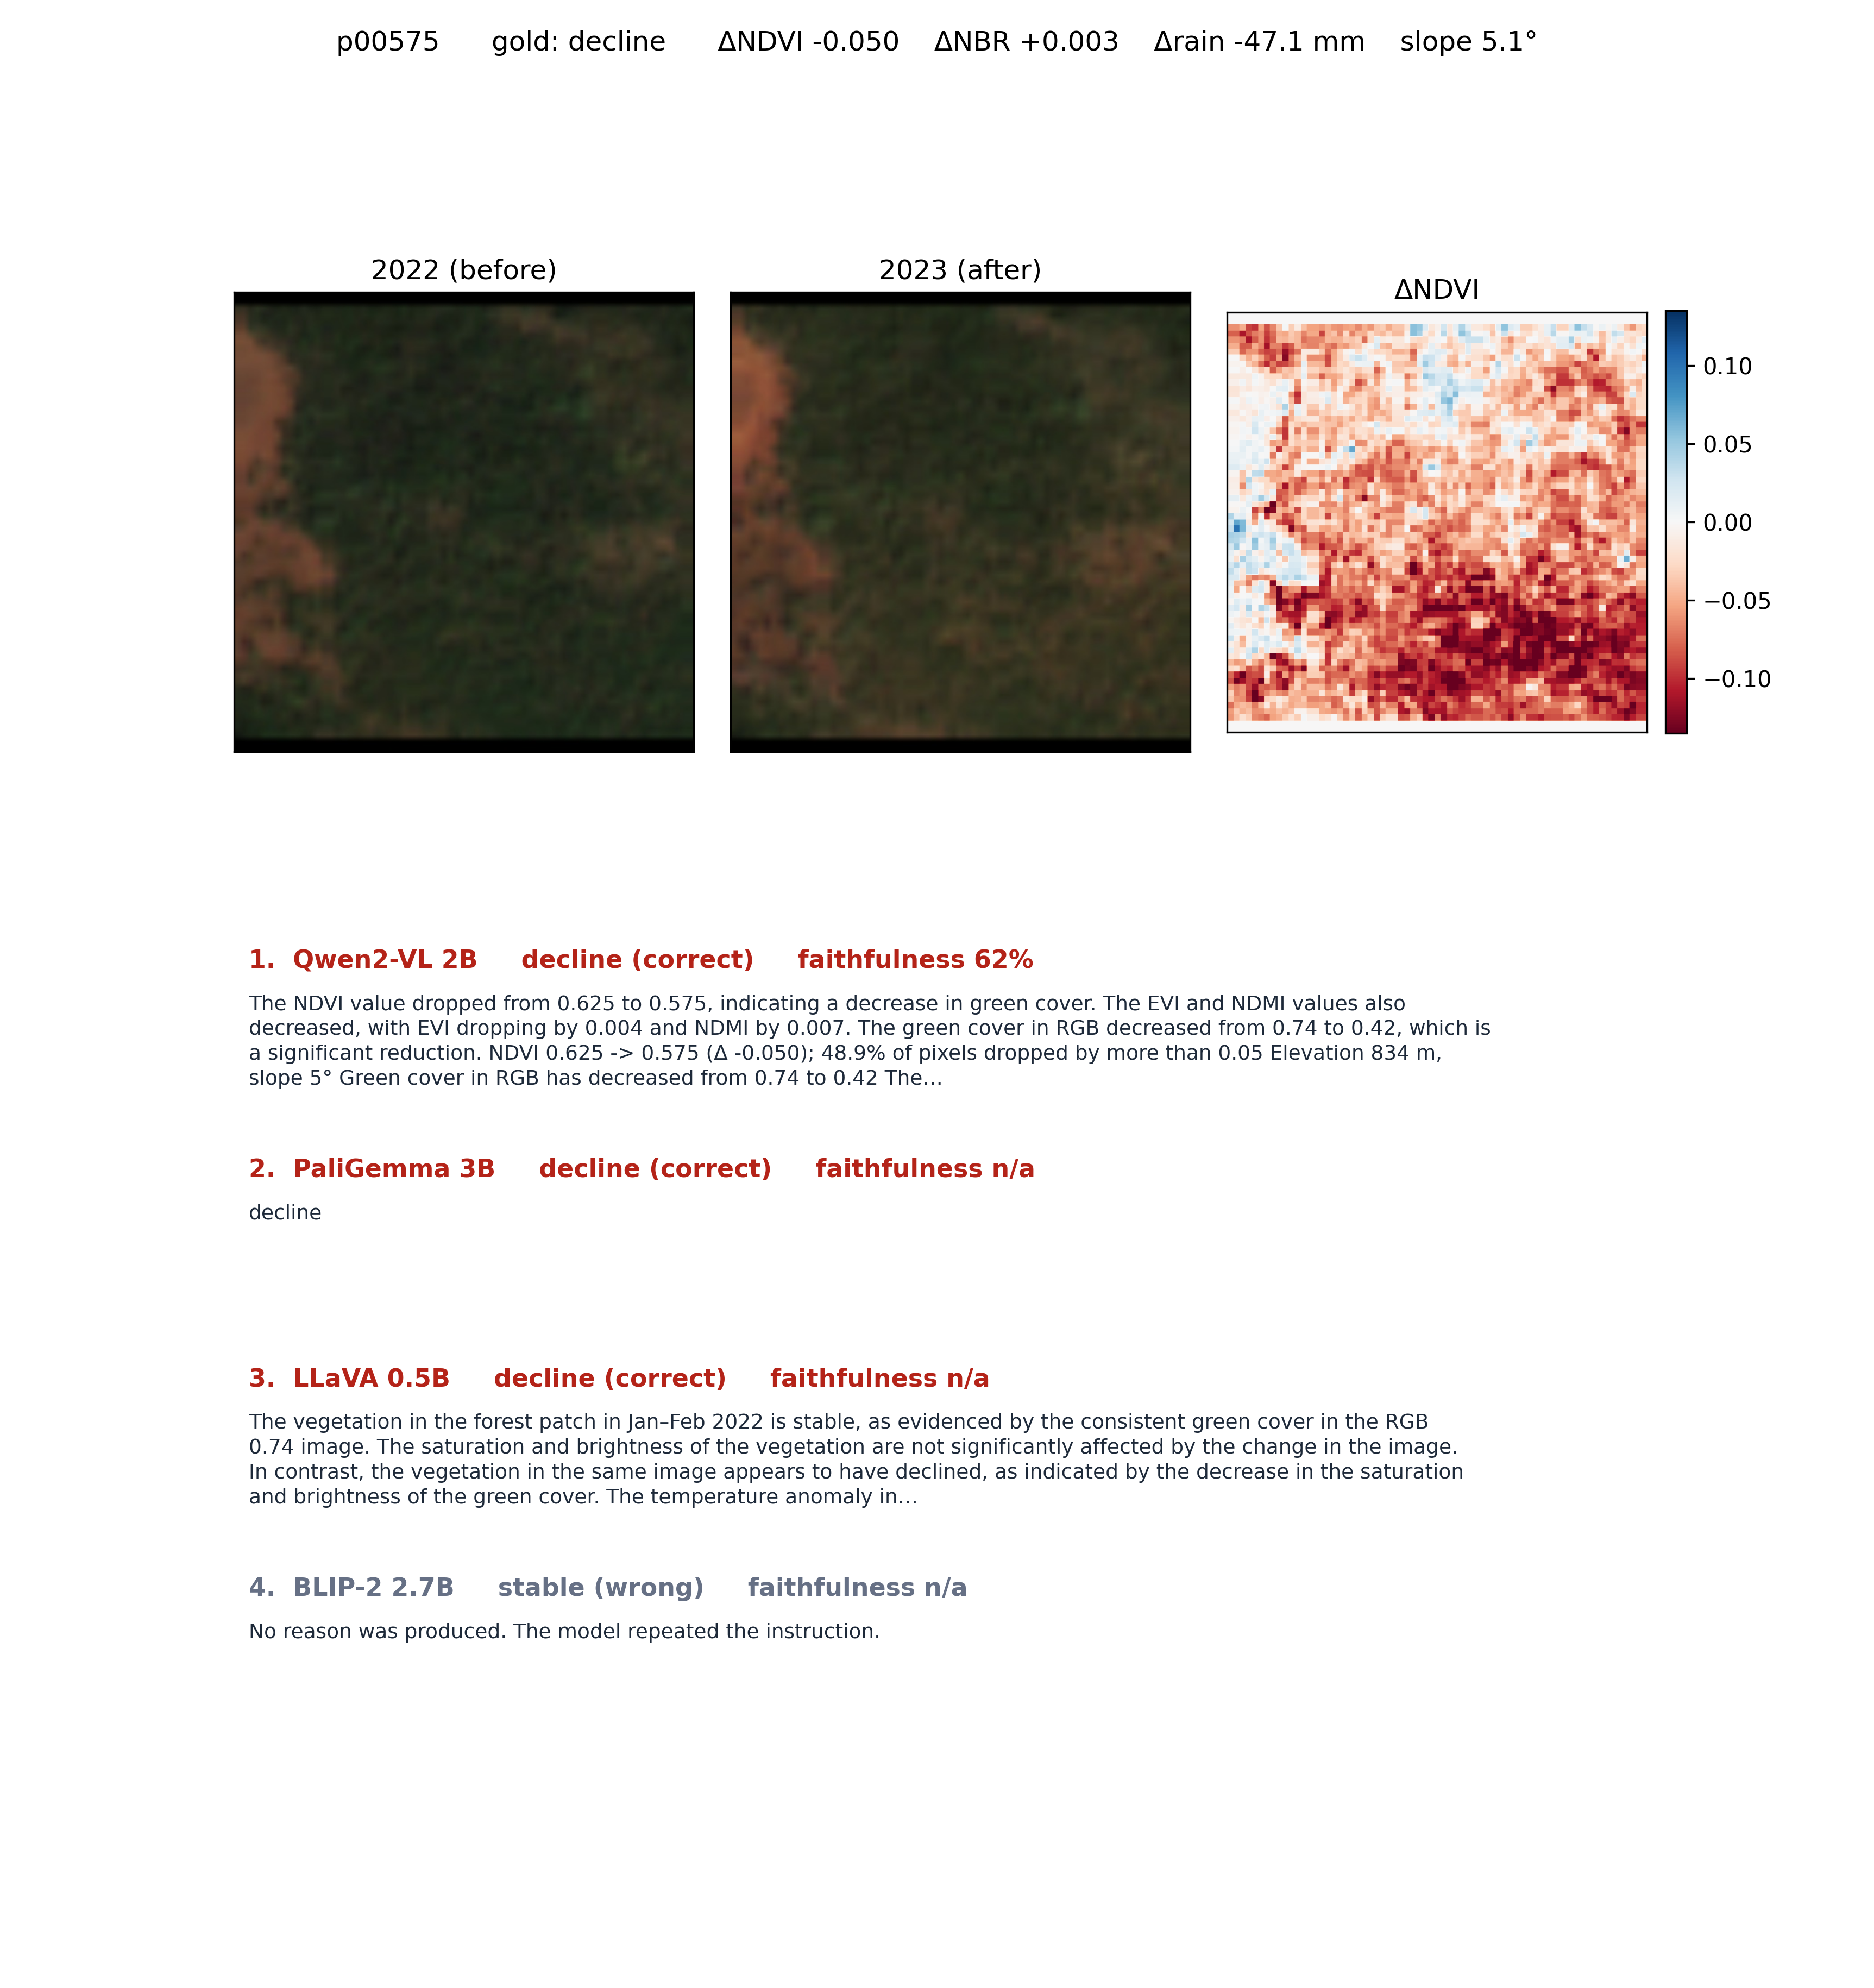
\includegraphics[width=0.74\textwidth]{figures/fig_panel_p00575.png}
\caption{Phase~B explanations for p00575 (gold \texttt{decline}, \dndvi{} $-0.050$), from \file{scripts/make_explanation_report.py}. Three models gave the right class; only Qwen gave a reason grounded in the numbers. The ``faithfulness'' heading in the panel is the project's name for claim correctness.}
\label{fig:panel}
\end{figure}

\section{Phase C: the structured cite-only prompt}
\label{sec:structured}

\subsection{Why it was added}

The free-form prompt gave models room to describe, interpret and speculate, and they used it badly: loops (LLaVA), invented climate causes (Qwen), echoed instructions (BLIP-2). The structured prompt removes that room. It asks the model to copy verified facts, apply a stated rule, and write one sentence about NDVI.

\subsection{What the model receives}

\begin{wherecode}
\file{src/vlm_evidence.py}: \texttt{evidence\_bullets}, \texttt{ndvi\_class\_hint}, \texttt{compact\_evidence\_structured}. \file{src/vlm_eval.py}: \texttt{EXPLAIN\_JSON\_ASK\_STRUCTURED}. \file{scripts/run_explain.py --prompt-style structured} writes \file{results/explain/explain_structured_<model>.json}.
\end{wherecode}

Under the compact table come two new blocks:
\begin{enumerate}
  \item \textbf{\texttt{ALLOWED\_FACTS}}: up to six numbered sentences built from the record, for example ``Patch mean NDVI was 0.625 in 2022 and 0.575 in 2023 ($\Delta$ $-0.050$).'', plus the EVI and NDMI changes, the rainfall totals, the temperature anomalies and the VV change. No class names.
  \item \textbf{\texttt{CLASS\_RULE}}: one line computed from that patch's NDVI change with $\pm0.02$ cut-offs, for example ``NDVI $\Delta \le -0.02 \rightarrow$ decline.'' It is not the \texttt{candidate\_class} field, but it does state a class for the patch.
\end{enumerate}

\begin{tcolorbox}[colback=gray!4,colframe=gray!50,fontupper=\scriptsize]
Images: 2022 (left/first) vs 2023 (right/second). Follow steps in order.\\
Step 1 --- Copy exactly 3 strings from ALLOWED\_FACTS (verbatim) into supporting\_evidence.\\
Step 2 --- Set change\_class using CLASS\_RULE and NDVI $\Delta$ only (stable, decline, or increase).\\
Step 3 --- Write justification as ONE sentence that mentions NDVI only; do not mention rainfall, temperature, or soil unless those lines were copied in Step 1.\\
Set conflicting\_evidence to [] and possible\_driver to "" (empty). Do not state causes or climate drivers.\\
Reply with JSON only: \{"visual\_change": "one short phrase", "change\_class": "stable|decline|increase", "justification": "...", "supporting\_evidence": ["...", "...", "..."], "conflicting\_evidence": [], "possible\_driver": "", "confidence": 0.5\}
\end{tcolorbox}

Only Qwen and LLaVA were run on all 55 test patches, on the MacBook Air's Apple GPU (\texttt{mps}) on 6 October: Qwen in 1,009\,s (18.3\,s per patch), LLaVA in 414\,s (7.5\,s per patch), up to 256 new tokens, greedy decoding.

\subsection{Results}

\begin{table}[H]
\centering
\caption{Phase~C on the 55 test patches (\file{results/explain/explanation_scores.csv}, 6 October; detailed counts recomputed from \file{explain_structured_*.json}).}
\label{tab:phaseC}
\small
\begin{tabular}{lrr}
\toprule
 & Qwen2-VL-2B & LLaVA-Interleave-0.5B \\
\midrule
Class accuracy (explanation mode) & 63.6\,\% (35/55) & 45.1\,\% (23 of 51 answered) \\
Class agrees with \texttt{CLASS\_RULE} & 53/55 & 42/55 \\
Output was complete JSON & 13/55 & 10/55 \\
\texttt{change\_class} left as the template text & 22/55 & 27/55 \\
Checkable claims per explanation & 2.85 & 2.33 \\
Correct claims & \textbf{75.8\,\%} (119/157) & \textbf{71.1\,\%} (91/128) \\
Explanations with $\ge 1$ claim flagged wrong & 36.4\,\% & 34.5\,\% \\
\quad of the flagged claims: change below the dead-band & 35 of 38 & 35 of 37 \\
\quad understatements / sign contradictions & 2 / 1 & 0 / 2 \\
Self-consistency & 100\,\% & 90.7\,\% \\
ROUGE-L against the evidence table & 0.566 & 0.250 \\
Distinct-2 / near-duplicate share & 0.21 / 9.1\,\% & 0.20 / 34.5\,\% \\
\bottomrule
\end{tabular}
\end{table}

\subsection{How to read them}

\paragraph{Claim correctness improved.} Qwen's correct claims rose from 43.8\,\% (3 patches) to 75.8\,\% (55 patches), LLaVA's from 56.7\,\% to 71.1\,\% (both on 55). LLaVA's self-consistency rose from 10\,\% to 91\,\%: its claims now point the same way as its class.

\paragraph{Most remaining ``errors'' are about tiny changes.} Of Qwen's 38 flagged claims, 35 describe a copied change smaller than the scorer's dead-band as a decrease or increase (for example ``EVI $\Delta$ $-0.006$'' or ``green cover 1.00 $\rightarrow$ 0.99''). These numbers are true; the scorer counts any change below 0.02 (0.05 for green cover) as stable. Only 1 Qwen claim and 2 LLaVA claims state the wrong sign. So the 36.4\,\% and 34.5\,\% of explanations ``with a wrong claim'' mostly reflect the strictness of the scorer, not invented facts.

\paragraph{The class comes from the stated rule.} Qwen's class matched \texttt{CLASS\_RULE} on 53 of 55 patches, and in 22 outputs the \texttt{change\_class} field was left as the template text, so the parser took the class from the copied rule. The rule alone scores 63.6\,\% against the labels, exactly Qwen's accuracy in this mode (Figure~\ref{fig:confusionA}f). This is instruction-following, not a new ability to classify.

\paragraph{Explanations became restatements.} ROUGE-L against the evidence table is 0.566 for Qwen, and many outputs repeat one fact: for p00701 all three ``supporting evidence'' items are ``NDVI 0.581 $\rightarrow$ 0.585 ($\Delta$ +0.004)''. LLaVA sometimes invents numbers in the allowed format: for p04508 it wrote ``NDVI $\Delta$ was +0.002'' when the change was $-0.005$. The direction check cannot catch this, because both values fall inside the ``stable'' dead-band.

\paragraph{Formatting.} Only 13 (Qwen) and 10 (LLaVA) outputs were complete JSON; the rest ran past the 256-token limit, mostly because the models copied the whole table. The parser still recovered a class for all Qwen outputs and 51 LLaVA outputs.

\begin{watchout}
\file{results/explain/explanation_scores.json} also contains ``structured'' rows for PaliGemma and BLIP-2 with 40\,\% accuracy. They come from a 5-patch test run on Ada (\texttt{n\_eval = 5}, zero checkable claims), and their source files are not on your laptop. Do not report them.
\end{watchout}

\section{Phase D: the explanation LoRA}
\label{sec:explora}

\subsection{The idea}

If a model sometimes writes good justifications, keep only the good ones and fine-tune the model on them, so that it writes good ones more often. This is a simple form of \emph{distillation}: a ``teacher'' model produces training targets for a ``student''. Here teacher and student are the same model, Qwen2-VL-2B (``2B-on-2B''), because the planned 7B teacher could not be downloaded: job 24225 failed in the download tool and job 24237 hit the disk quota of the Ada home directory.

\subsection{Step 1: building the targets (Ada job 24298)}

\begin{wherecode}
\file{scripts/build_explain_targets.py} and \file{scripts/ada_slurm_explain_targets.sh}. Output: \file{data/explain_targets/train_targets.jsonl} and \file{results/explain/target_filter_report.json}; log \file{results/slurm-explain-targets-24298.log}.
\end{wherecode}

For each of the 256 training patches, the teacher received the label-free compact table and the free-form JSON prompt of Phase~B (up to 256 new tokens). A justification was kept only if (i) its class equalled the label, (ii) it contained at least two checkable claims, and (iii) \emph{all} its claims agreed with the measured changes. \textbf{28 of 256} passed.

\begin{newinfo}
Looking inside \file{train_targets.jsonl} (recomputed for this guide):
\begin{itemize}
  \item The 28 kept targets are \textbf{26 decline, 2 increase and 0 stable}. A filter that requires the class to be right keeps the cases the teacher already handled, and the 2B teacher was mostly right about declines.
  \item In \textbf{12 of the 28}, the \texttt{justification} field holds the teacher's raw output, starting with a code fence (\verb|```json|) and cut off mid-sentence, because the parser could not read the truncated JSON and fell back to the raw text. The student was trained to reproduce these nested, unfinished outputs.
\end{itemize}
\end{newinfo}

\subsection{Step 2: training (Ada job 24389)}

\texttt{python scripts/run\_finetune\_qwen.py --train --eval --target explain --max-train 128 --epochs 1}, with the same LoRA settings as Track~B and the label-free table as input. Because \texttt{--max-train 128} keeps the first 128 training patches by ID, only \textbf{16 of the 28 targets} were used (the log prints ``explain targets kept 16 / 128''). Those 16 are \textbf{all labelled decline}, and 9 of them are the raw, cut-off kind. The single epoch was kept by development accuracy measured in one-word \texttt{evidence\_only} mode (34.5\,\%, the majority level), so the selection step chose nothing in practice.

\subsection{Step 3: testing}

The adapter was tested on the 55 test patches in explanation mode, with the label-free table and the free-form JSON prompt (935\,s). Results (\file{results/explain/explain_qwen_vl_finetuned_ecoexplain.json}, \file{explanation_scores.json}):

\begin{table}[H]
\centering
\caption{Phase~D on the 55 test patches. Interval, macro-F1, confusion and rule agreement recomputed for this guide.}
\label{tab:phaseD}
\small
\begin{tabular}{L{6.0cm}L{8.2cm}}
\toprule
Targets kept by the filter / used in training & 28 of 256 / 16 (all decline) \\
Class accuracy (explanation mode) & \textbf{61.8\,\%} (34/55; 95\,\% interval 48.6--73.5\,\%) \\
Macro-F1 & 0.525 \\
Per class & decline 17/18, stable 0/18 (all called decline), increase 17/19 \\
Answers that match the $\pm0.02$ NDVI rule & 28/55 \\
Checkable claims per explanation & 6.84 \\
Correct claims & 50.5\,\% \\
Explanations with $\ge 1$ wrong claim & 74.5\,\% \\
Self-consistency & 96.4\,\% \\
ROUGE-L against the evidence table & 0.205 \\
\bottomrule
\end{tabular}
\end{table}

\subsection{How to read it}

\begin{itemize}
  \item \textbf{It is not a better explainer.} Claim correctness (50.5\,\%) is lower than structured zero-shot Qwen (75.8\,\%), and three explanations in four contain at least one wrong claim. The student writes many more claims (6.84 per explanation, because its targets included long evidence lists), and more of them are wrong.
  \item \textbf{Its class answers are not comparable with Track~A.} 61.8\,\% comes from a JSON explanation written from the label-free table, after training on 16 justifications; Track~A scores one-word answers. Like the first class LoRA, it calls every stable patch ``decline'' (Figure~\ref{fig:loraclasses}d), and with 16 decline-only targets it could hardly learn otherwise.
  \item \textbf{But it does separate decline from increase.} It was right on 17 of 18 decline and 17 of 19 increase patches, without the label line and without a stated rule. Against always answering ``increase'' that is significant (McNemar: 17 gained, 2 lost, $p < 0.001$), the only label-free classification in the project that is. Two cautions: it never answers ``stable'', and zero-shot Qwen was run in this free-form explanation mode on only 3 patches, so you cannot tell whether the LoRA or the prompt (which asks the model to cite the numbers) produced it. Running zero-shot Qwen in the same mode on all 55 patches would settle it.
  \item \textbf{What it shows.} The pipeline for teacher filtering and explanation fine-tuning works end to end, and a 2B teacher is too weak to produce useful targets: it passed only 28 of 256, almost all of one class. That is a useful pilot result with a clear next step (a stronger teacher, balanced targets, clean JSON).
\end{itemize}

\begin{watchout}
Do not put 61.8\,\% in the same table as 56.4\,\% and 67.3\,\%. Those are one-word classifications with the full card; 61.8\,\% is the class parsed from a JSON explanation written from a label-free table after training on 16 justifications.
\end{watchout}

\section{All explanation phases together}

\begin{figure}[H]
\centering
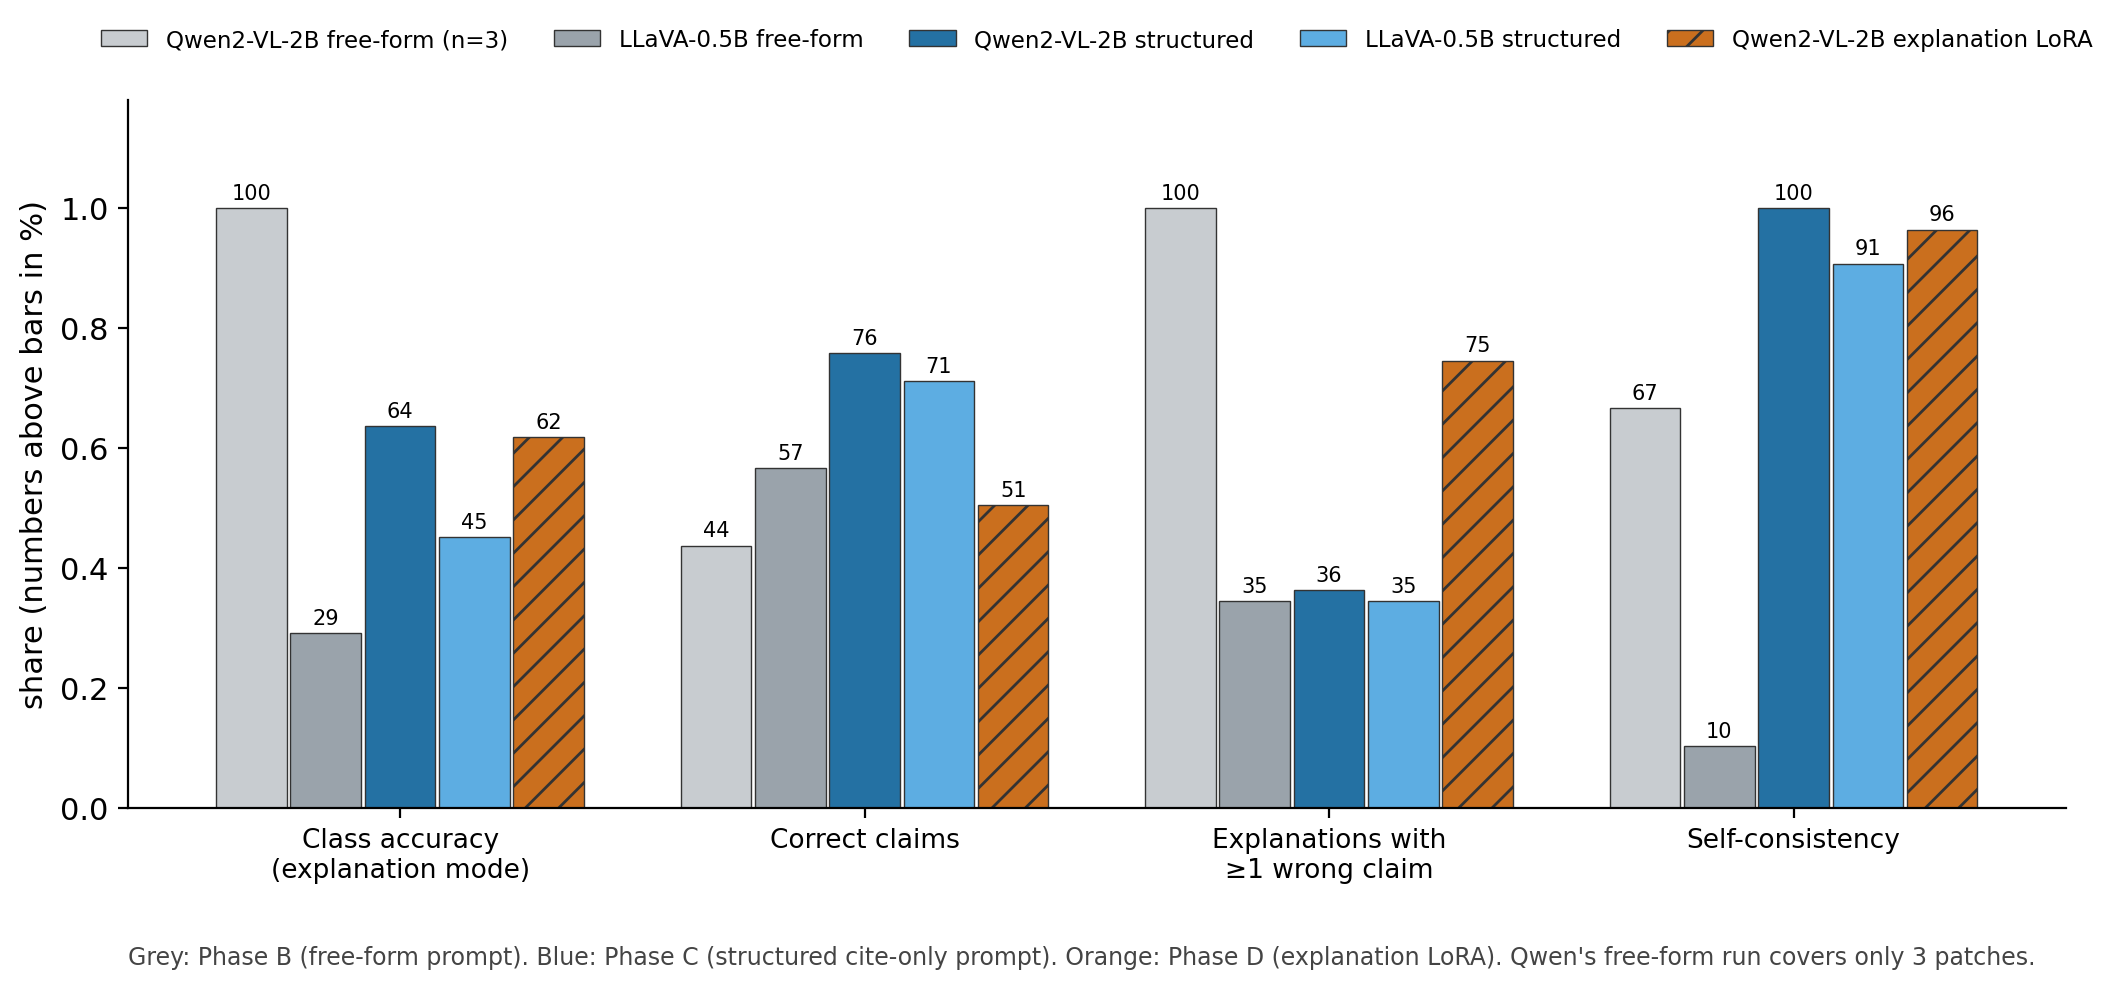
\includegraphics[width=\textwidth]{figures/fig_explain_phases.png}
\caption{Explanation scores across the three phases. Grey: free-form prompt (Qwen on 3 patches only). Blue: structured cite-only prompt. Orange: explanation LoRA. Phase~B values from \texttt{score\_explanations.py --include-legacy}; Phase~C from \file{explanation_scores.csv}; Phase~D from \file{explanation_scores.json}. Made by \file{study_guide_v2/make_figures_v2.py}.}
\label{fig:explphases}
\end{figure}

\begin{plainwords}
The pattern is clear. Free text from small models is unreliable. Telling them exactly which facts they may use makes their claims mostly correct, but then they mostly repeat those facts and follow the stated rule. Fine-tuning on a handful of self-made justifications did not help: it produced longer explanations with more wrong claims.
\end{plainwords}

\begin{newinfo}
\textbf{Which file holds which number.} \file{results/explain/explanation_scores.csv} (6 October) holds the Phase~B rows that were kept and the Phase~C rows (Qwen and LLaVA structured). \file{results/explain/explanation_scores.json} was overwritten on 17 October by the Ada run and now holds Phase~D (plus the two 5-patch rows above). The Phase~B values for Qwen and LLaVA come from \texttt{scripts/score\_explanations.py --include-legacy}. If you re-run the scorer, both files will change: copy them first.
\end{newinfo}

\begin{foryourreport}
In ``Explanation Quality'' (about 900 words):
\begin{itemize}
  \item What the models received (label-free table; \file{check_no_leak.py}) and the two prompts, briefly (prompts in an appendix).
  \item Phase~B in a few sentences per model, with one short example (p00086 or p00575).
  \item Phase~C: Table~\ref{tab:phaseC} (shortened); the dead-band finding; the class follows the stated rule (53/55, ceiling 63.6\,\%); the restatement trade-off.
  \item Phase~D: the 28/256 filter, the 16 decline-only targets, the results, and why it is a pilot.
  \item Figure~\ref{fig:explphases} as the summary.
  \item One sentence on what the scorer measures (evidence consistency) and its limits \citep{jacovi2020,turpin2023}.
\end{itemize}
\end{foryourreport}

\begin{selfcheck}
\begin{enumerate}
  \item What did the models receive in explanation mode instead of the full card, and why?
  \item Describe one failure of each model under the free-form prompt.
  \item What are \texttt{ALLOWED\_FACTS} and \texttt{CLASS\_RULE}?
  \item Why are most of the ``wrong'' claims in Phase~C not really wrong?
  \item Why is Qwen's 63.6\,\% in Phase~C not evidence of better classification?
  \item Give three reasons why the explanation LoRA did not produce better explanations.
  \item Why must 61.8\,\% not be compared with 56.4\,\%?
\end{enumerate}
\end{selfcheck}
